\section{Acceptance and efficiency systematics}
\label{sec:systematics}

This is a search for new physics contributions to 
events with high \met and lots of jet activity.
As seen in Section~\ref{sec:results}, there is no
evidence for a contribution beyond SM expectations.

Strictly speaking it is impossible to talk about 
``acceptance and efficiency systematics'' because these kinds of
systematics only apply to a well defined final state.
Nevertheless, we can make general statements about the 
systematic uncertainties, including quantitative
estimates of the systematic uncertainties associated with
a few specific processes. 
% Note that we have used Spring10 
% MC for the studies of systematic uncertainties described in this section,
% and we are currently checking if any of the reported values
% change after switching to Fall10 MC.

The systematic uncertainty on the lepton acceptance consists
of two parts: the trigger efficiency uncertainty and the 
ID and isolation uncertainty.  We discuss these in turn.

The trigger efficiency 
for two leptons of $P_T>10$ GeV, with one lepton of 
$P_T>20$ GeV is very high, except in some corners
of phase space, see Section~\ref{sec:trgeffsum}. 
We estimate the efficiency uncertainty to be a few percent,
mostly in the low $P_T$ region. For $t\bar{t}$, LM0 and LM1
we find trigger efficiency uncertainties of less than 1\%, evaluated
by taking the difference in yields in the signal region between
assuming 100\% trigger efficiency and using the trigger efficiency model.
% trigger efficiency uncertainties: ttbar 0.3%, LM0 0.6%, LM1 0.6%

\begin{figure}[tbh]
\begin{center}
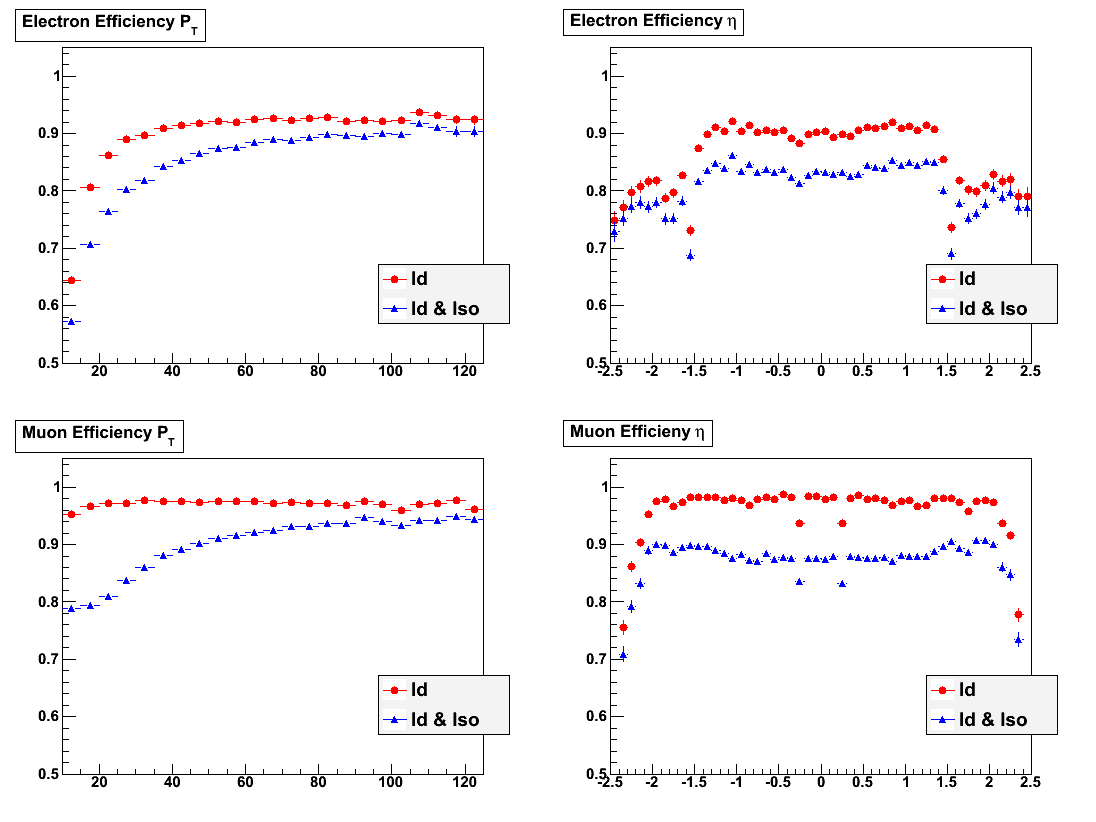
\includegraphics[width=1.0\linewidth]{ttdilD6T_eff_Dec02_38X.png}
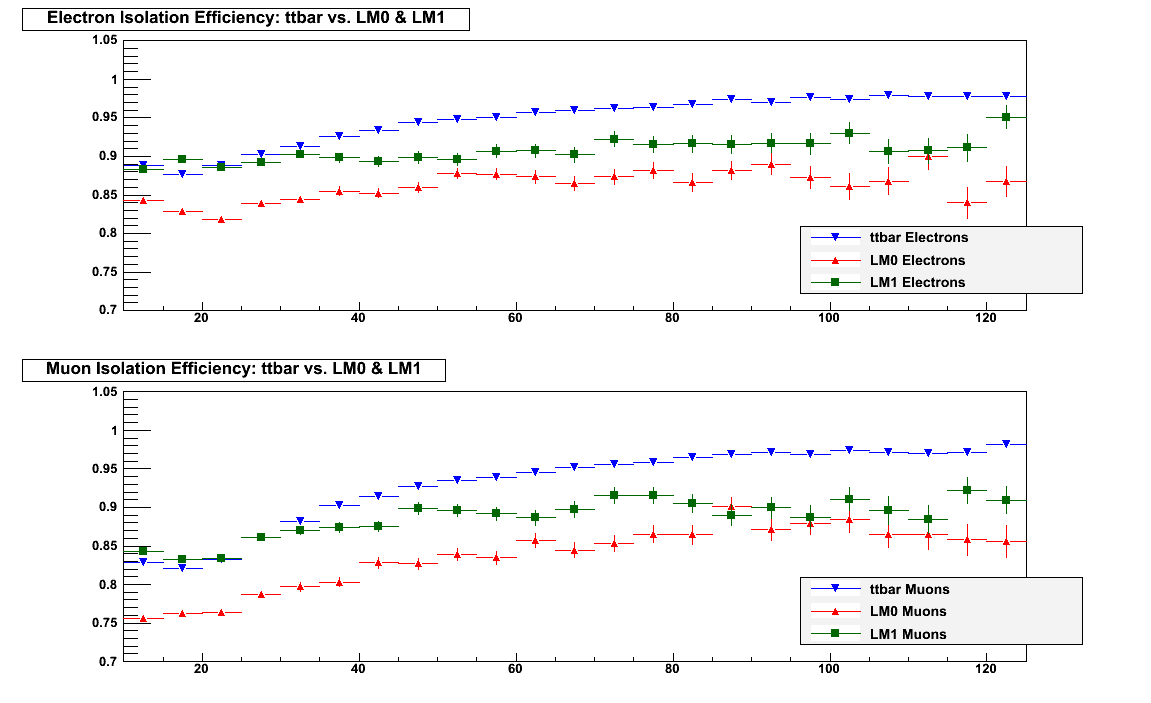
\includegraphics[width=1.0\linewidth]{lm_eff_Dec02_38X.png}
\caption{\label{fig:effttbar}\protect 
Identification and isolation efficiencies for leptons from $t \to W \to \ell$ and 
$t \to W \to \tau \to \ell$ in $t\bar{t}$ events (top). Isolation efficiency
for $t\bar{t}$, LM0 and LM1 (bottom).}
\end{center}
\end{figure}


\begin{table}[hbt]
\begin{center}
\caption{\label{tab:tagandprobe} Tag and probe results on $Z \to \ell \ell$
on data and MC.  We quote ID efficiency given isolation and 
the isolation efficiency given ID. }
\begin{tabular}{|l||c|c|}
\hline
                             & Data  T\&P      & MC T\&P             \\  
\hline
$\epsilon(id|iso)$ electrons & $0.925 \pm 0.007$ & $0.934 \pm 0.004$ \\
$\epsilon(iso|id)$ electrons & $0.991 \pm 0.002$ & $0.987 \pm 0.002$ \\
$\epsilon(id|iso)$ muons     & $0.962 \pm 0.005$ & $0.984 \pm 0.002$ \\
$\epsilon(iso|id)$ muons     & $0.987 \pm 0.003$ & $0.982 \pm 0.002$ \\ 
\hline
\end{tabular}
\end{center}
\end{table}


The ID efficiencies in MC are shown in 
Figures~\ref{fig:effttbar}
for the leptons from $t \to W \to \ell$ and $t \to W \to \tau \to \ell$.
Tag and probe studies show that these are correct to about 2\%,
see Table~\ref{tab:tagandprobe}.
Note that the isolation efficiency depends on the jet activity in
the final state.  For example, in MC we find that the
lepton isolation efficiency differs by $\approx 4\%$ 
{\bf per lepton} between $Z$ events and $t\bar{t}$ events\cite{ref:top}.
%\noindent {\bf This figure should be cut off at 100 GeV, and 
%the y-axis should be zero-suppressed}

Another significant source of systematic uncertainty is 
associated with the jet and $\met$ energy scale.  The impact
of this uncertainty is final-state dependent.  Final
states characterized by lots of hadronic activity and \met are 
less sensitive than final states where the \met and SumJetPt
are typically close to the requirement.  To be more quantitative,
we have used the method of Reference~\cite{ref:top} to evaluate
the systematic uncertainties on the acceptance for $t\bar{t}$ 
and two benchmark SUSY points.  The uncertainties are calculated
assuming a 5\% uncertainty to the hadronic energy scale in CMS.

For $t\bar{t}$ we find uncertainties of 8\% (baseline 
selection) and 27\% (signal region D); for LM0 and LM1 we find
14\% and 6\% respectively for signal region D.

\clearpage